\documentclass{beamer}
\usetheme{Madrid}
% Abilita il supporto alle immagini
\usepackage{graphicx}
%Path relative to the main .tex file 
\graphicspath{ {./images/} }
\usepackage{fancybox}

% Informazioni da includere nella pagina del titolo:
\title[DCC performance in IEEE 802.11p] % opzionale
{On the performance of Decentralized Congestion Control in a real IEEE 802.11p testbed}

\author{\textbf{Antonio Solida - 17850}}

\institute[] % opzionale
{
    \textbf{Relatore: Prof. Carlo Augusto Grazia}
    \and
    Corso di Laurea Magistrale in Ingegneria Informatica\\
    Percorso "Cloud \& Cybersecurity"\\
    Esame di Automotive Connectivity
    \and
    Dipartimento di Ingegneria "Enzo Ferrari"\\
    Università degli studi di Modena e Reggio Emilia
}

\date[17 ottobre 2024] % opzionale
{Modena, (forse) 17 ottobre 2024}

\begin{document}

\frame{\titlepage}

\begin{frame}
\frametitle{Introduzione}
\begin{columns}
    % Column 2    
    \begin{column}{0.5\textwidth}
        \begin{figure}[h!]
            \centering
            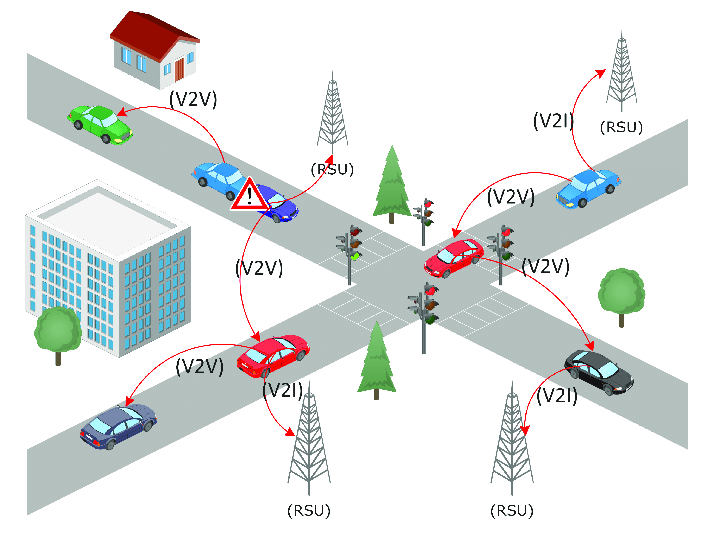
\includegraphics[width=1\textwidth]{vanet.png}
            \label{fig:vanet}
        \end{figure}
    \end{column}
    \begin{column}{0.5\textwidth}
        \begin{figure}[h!]
            \centering
            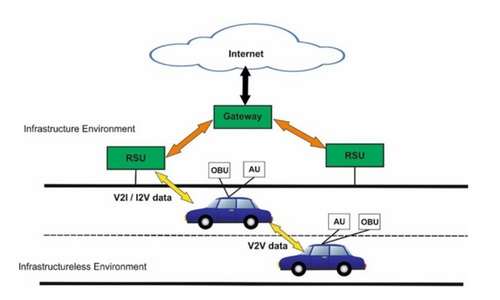
\includegraphics[width=1\textwidth]{routing_vanet.jpeg}
            \label{fig:obu_rsu}
        \end{figure}
    \end{column}
\end{columns}
\end{frame}

\begin{frame}
    \frametitle{Problema della congestione}
\end{frame}

\begin{frame}
    \frametitle{DCC con QoS}
\end{frame}

\begin{frame}
    \frametitle{Descrizione testbed}
    \centering
    % Aggiunta dell'immagine del diagramma
    \begin{minipage}{0.6\textwidth}
        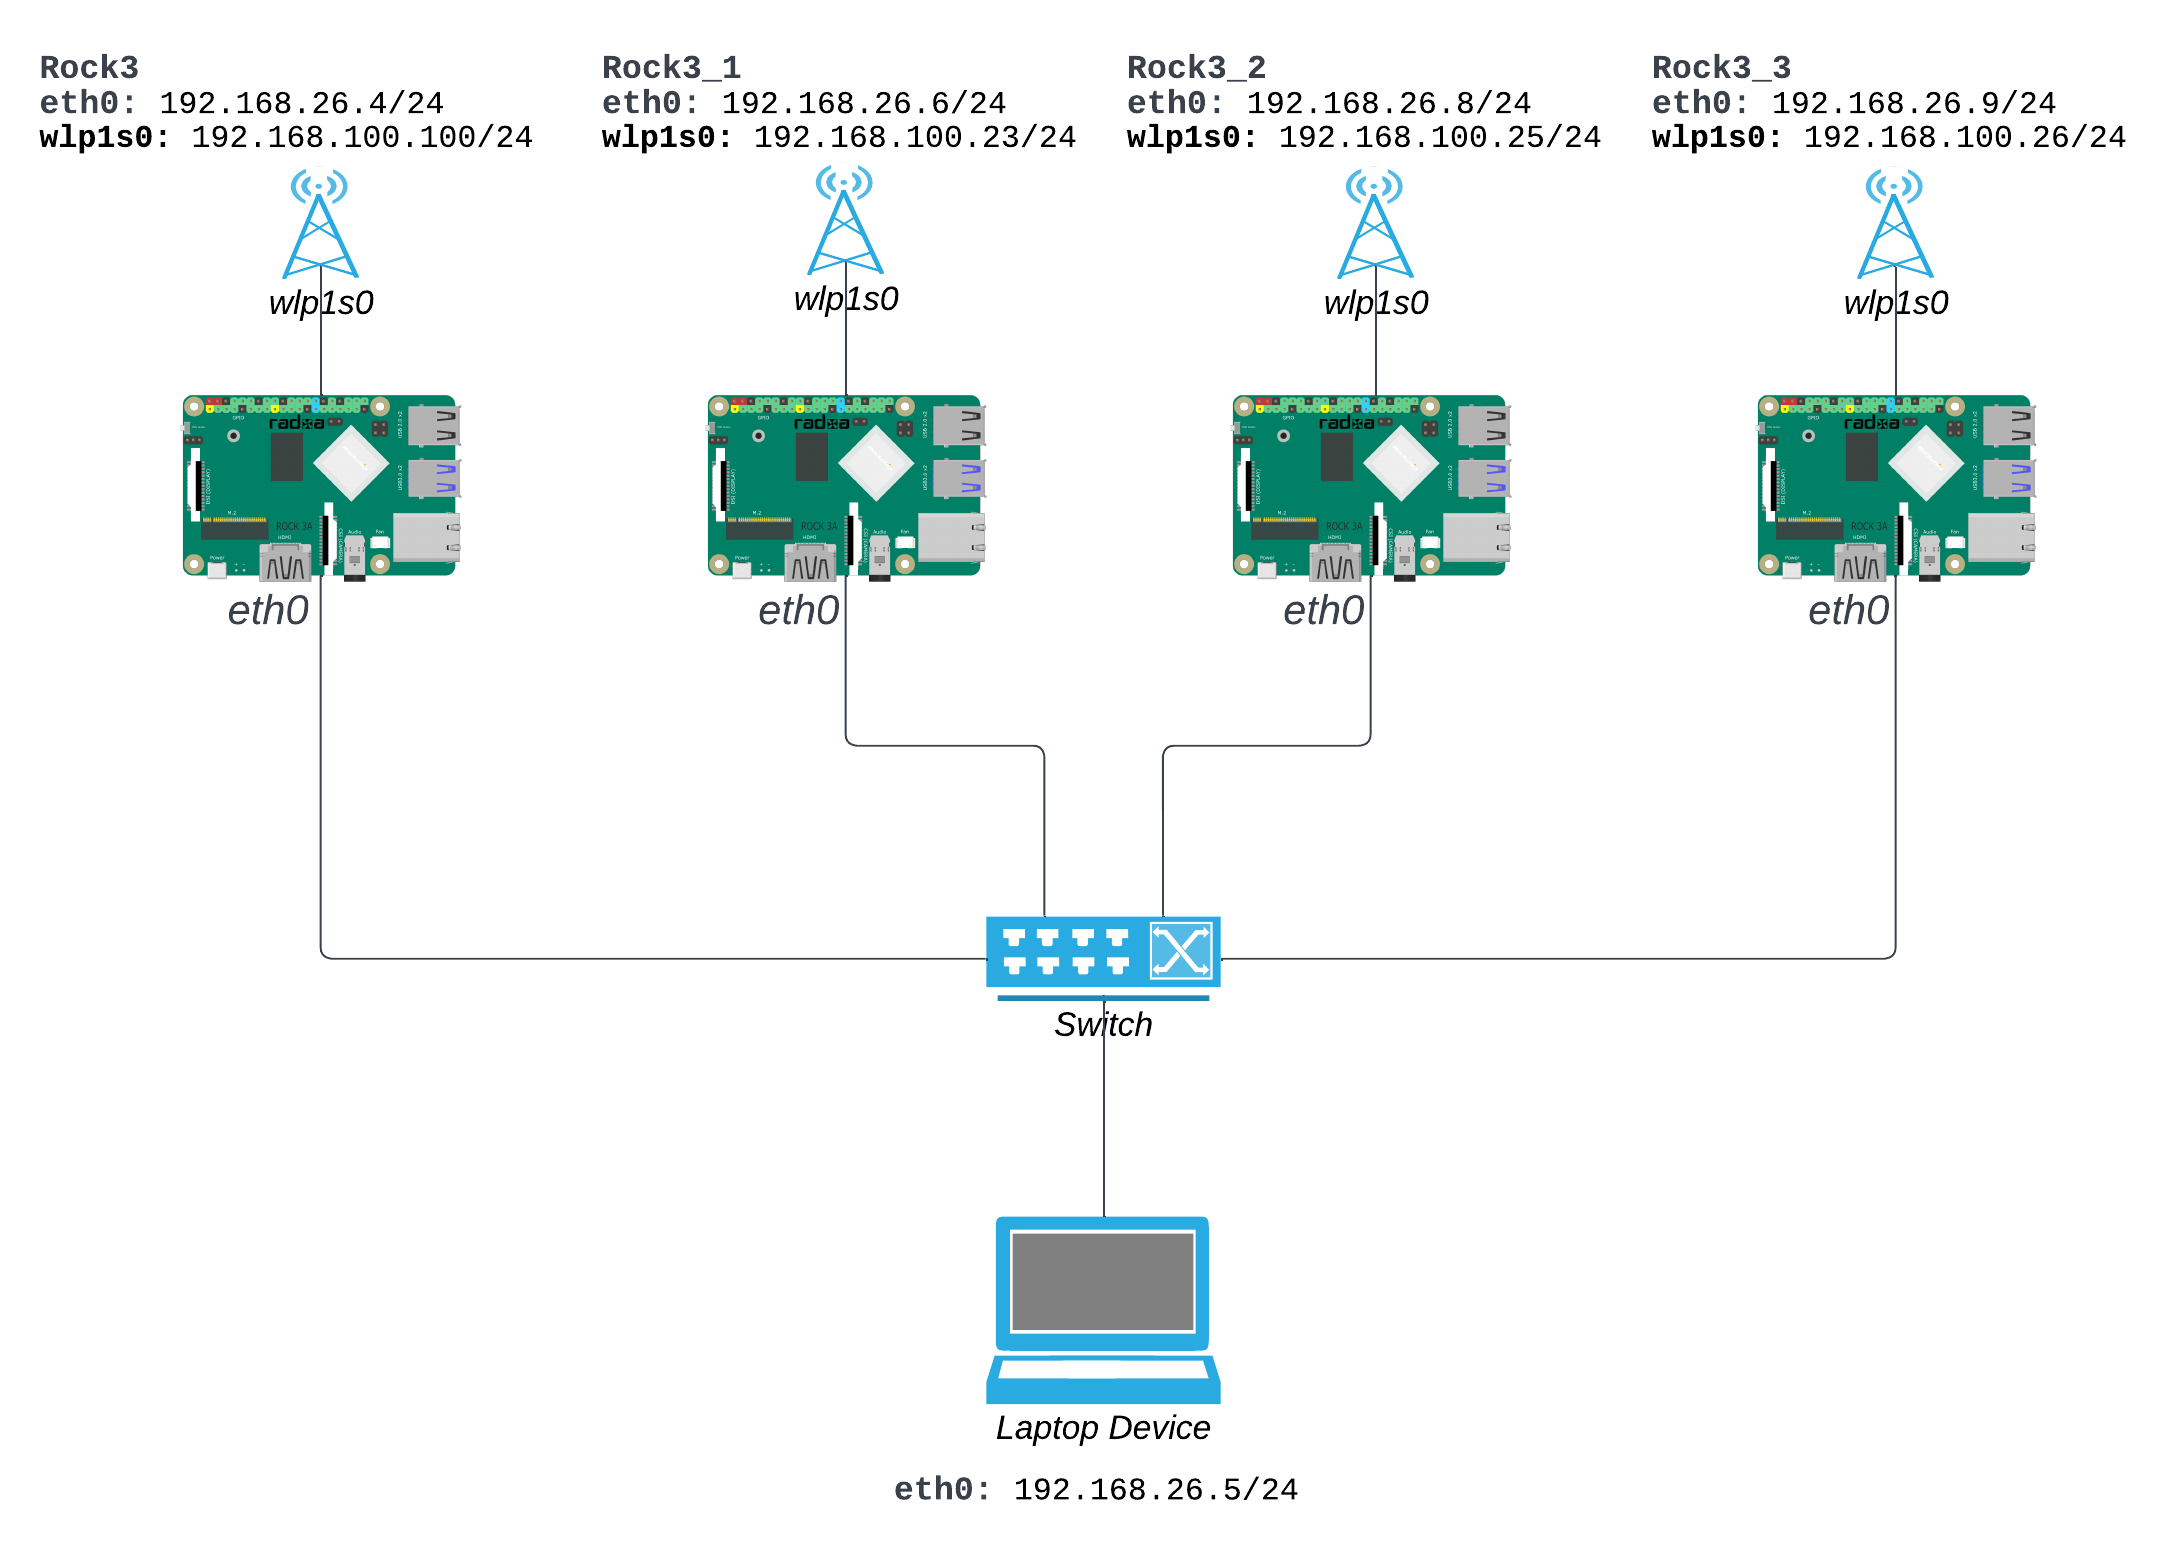
\includegraphics[width=\textwidth]{topology.png} % Sostituisci con il path della tua immagine
    \end{minipage}
    \hfill
    % Aggiunta dell'immagine della scheda e del laptop
    \begin{minipage}{0.35\textwidth}
        \centering
        % Immagine della scheda Rock 3A
        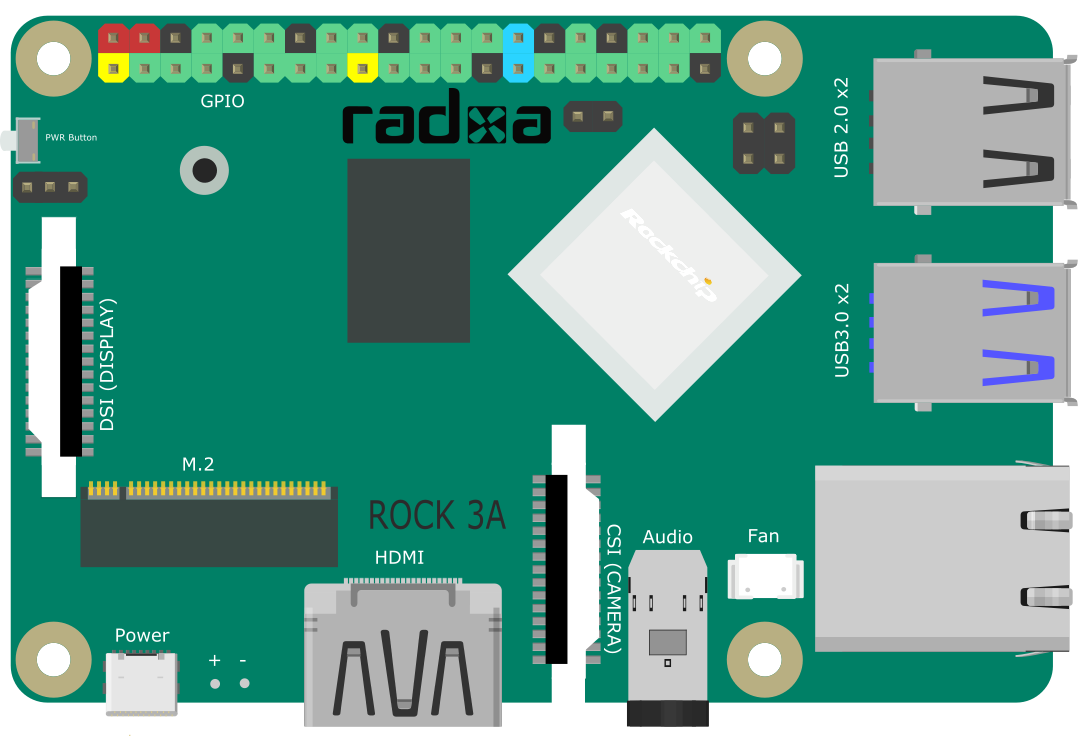
\includegraphics[width=\textwidth]{ROCK_3A.png} % Sostituisci con il path della tua immagine
        \vspace{0.5cm}
        % Immagine del laptop
        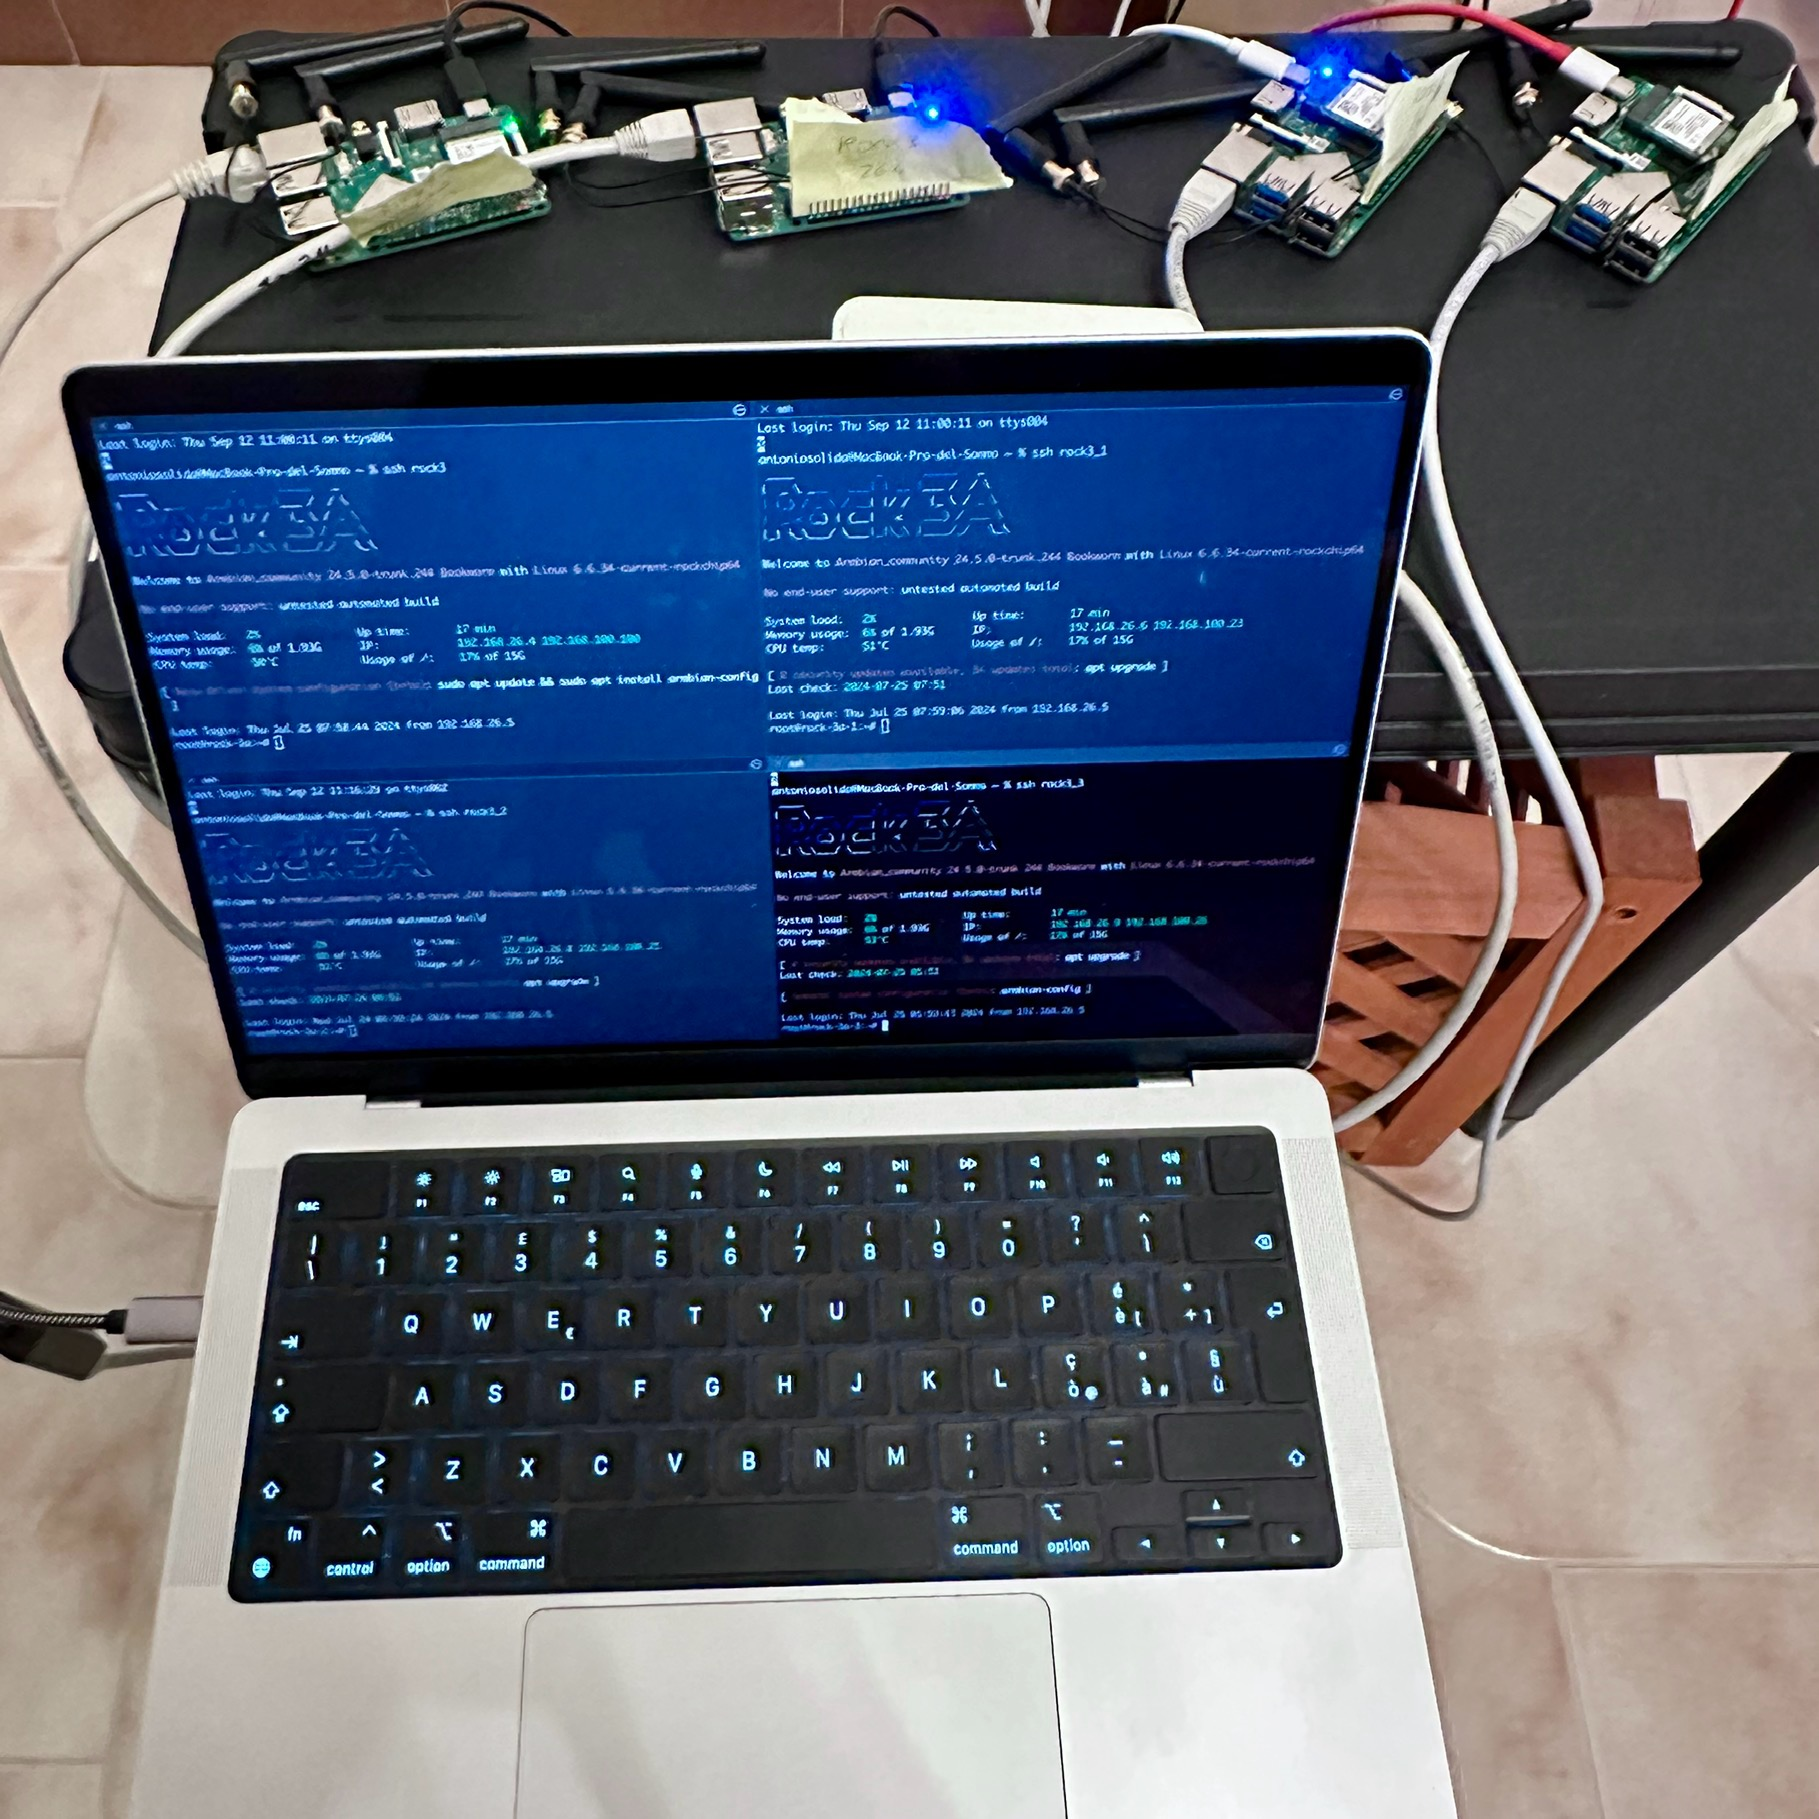
\includegraphics[width=\textwidth]{topology_photo.jpg} % Sostituisci con il path della tua immagine
    \end{minipage}
\end{frame}

\begin{frame}
    \frametitle{Descrizione test}
    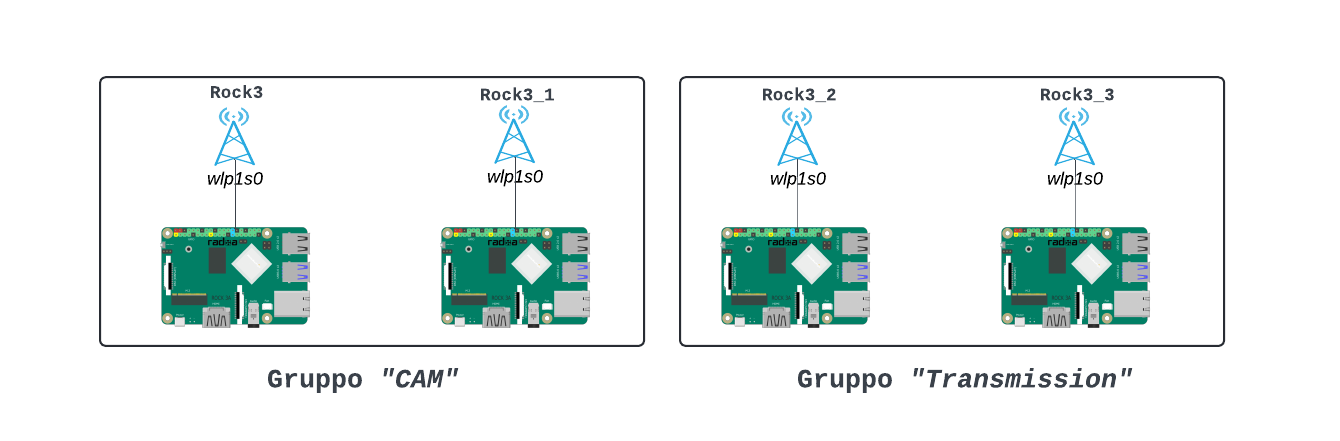
\includegraphics[width=\textwidth]{Rock scheme.png}
\end{frame}

\begin{frame}
    \frametitle{Trasmissione in ambiente non congestionato}
    
    \begin{minipage}{0.45\textwidth}
        \textbf{Quality of Service assente}\\
        \textit{Throughput medio Stream ID 1}: 3.49 Mbps\\
        \textit{Throughput medio Stream ID 2}: 3.47 Mbps\\
        \vspace{1cm}
        
        \textbf{Quality of Service presente}\\
        \textit{Throughput medio Stream ID 1 (AC\_VO)}: 7.96 Mbps\\
        \textit{Throughput medio Stream ID 2 (AC\_BK)}: 0.61 Mbps\\
    \end{minipage}
    \hfill
    \begin{minipage}{0.5\textwidth}
        \centering
        \begin{minipage}{\textwidth}
            % Primo grafico (Quality of Service assente)
            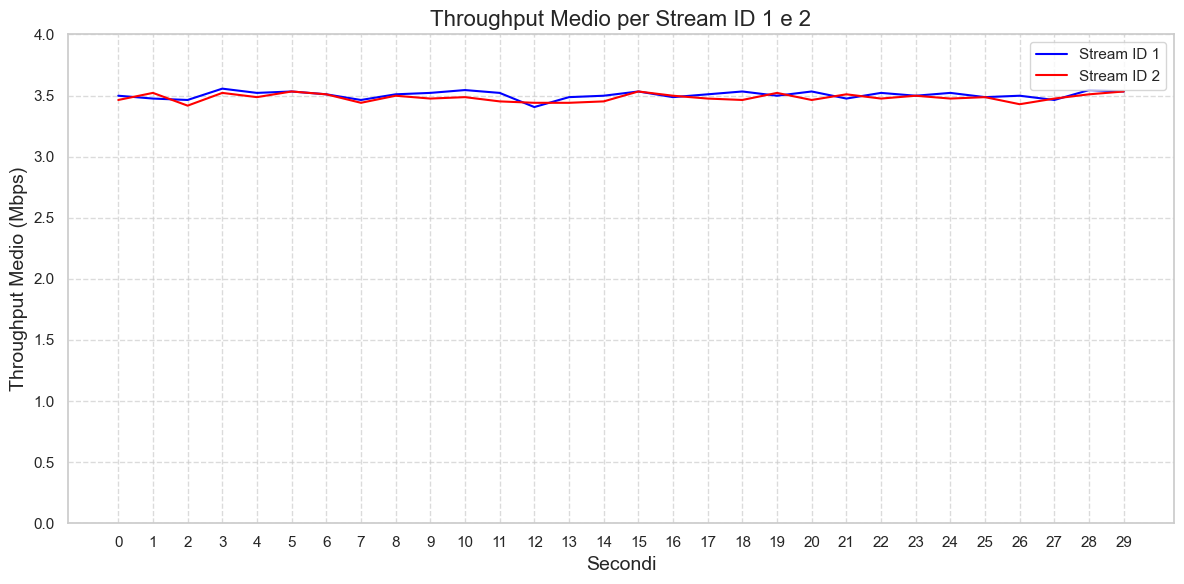
\includegraphics[width=\textwidth]{t1_c0_main.png} % Sostituisci con il path del grafico
            \vspace{0.5cm}
        \end{minipage}
        \begin{minipage}{\textwidth}
            % Secondo grafico (Quality of Service presente)
            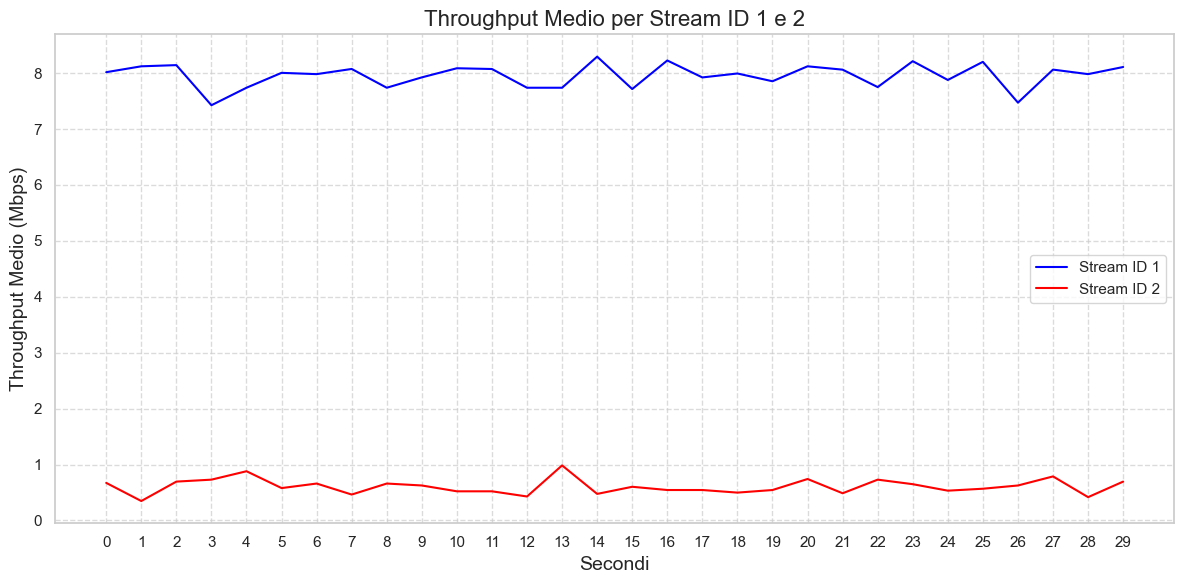
\includegraphics[width=\textwidth]{t2_c0_main.png} % Sostituisci con il path del grafico
        \end{minipage}
    \end{minipage}

\end{frame}


\begin{frame}
    \frametitle{Trasmissione in ambiente parzialmente congestionato}
    
    \begin{minipage}{0.45\textwidth}
        % Quality of Service assente
        \textbf{Quality of Service assente}\\
        \textit{Throughput medio Stream ID 1}: 3.13 Mbps\\
        \textit{Throughput medio Stream ID 2}: 3.13 Mbps\\
        
        \vspace{1cm}
        
        % Quality of Service presente
        \textbf{Quality of Service presente}\\
        \textit{Throughput medio Stream ID 1 (AC\_VO)}: 6.73 Mbps\\
        \textit{Throughput medio Stream ID 2 (AC\_BK)}: 0.77 Mbps\\
    \end{minipage}
    \hfill
    \begin{minipage}{0.5\textwidth}
        \centering
        \begin{minipage}{\textwidth}
            % Primo grafico (Quality of Service assente)
            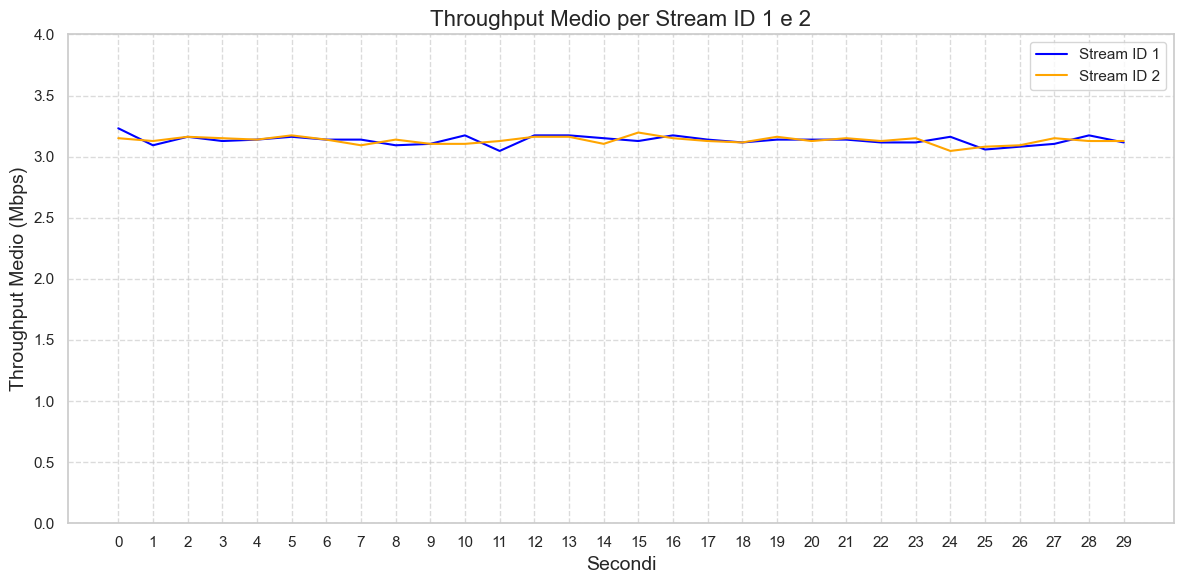
\includegraphics[width=\textwidth]{t1_c1_main.png} % Sostituisci con il path del grafico
            \vspace{0.5cm}
        \end{minipage}
        \begin{minipage}{\textwidth}
            % Secondo grafico (Quality of Service presente)
            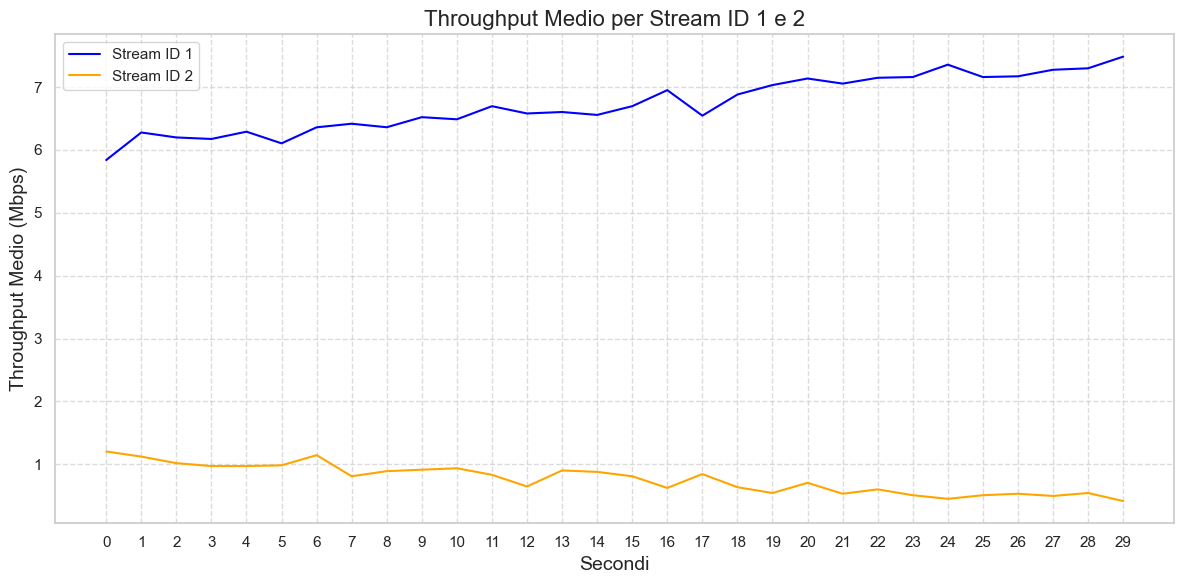
\includegraphics[width=\textwidth]{t2_c1_main.png} % Sostituisci con il path del grafico
        \end{minipage}
    \end{minipage}

\end{frame}

\begin{frame}
    \frametitle{Trasmissione in ambiente totalmente congestionato}
    
    \begin{minipage}{0.45\textwidth}
        % Quality of Service assente
        \textbf{Quality of Service assente}\\
        \textit{Throughput medio Stream ID 1}: 1.14 Mbps\\
        \textit{Throughput medio Stream ID 2}: 1.19 Mbps\\
        
        \vspace{1cm}
        
        % Quality of Service presente
        \textbf{Quality of Service presente}\\
        \textit{Throughput medio Stream ID 1 (AC\_VO)}: 6.19 Mbps\\
        \textit{Throughput medio Stream ID 2 (AC\_BK)}: 0.30 Mbps\\
    \end{minipage}
    \hfill
    \begin{minipage}{0.5\textwidth}
        \centering
        \begin{minipage}{\textwidth}
            % Primo grafico (Quality of Service assente)
            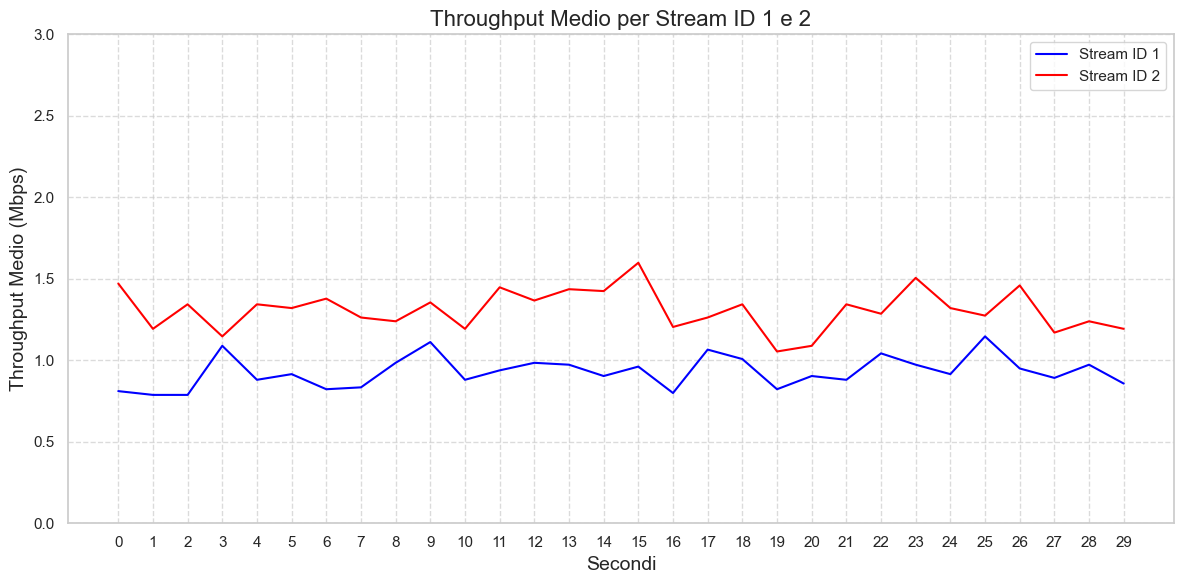
\includegraphics[width=\textwidth]{t1_c2_main.png} % Sostituisci con il path del grafico
            \vspace{0.5cm}
        \end{minipage}
        \begin{minipage}{\textwidth}
            % Secondo grafico (Quality of Service presente)
            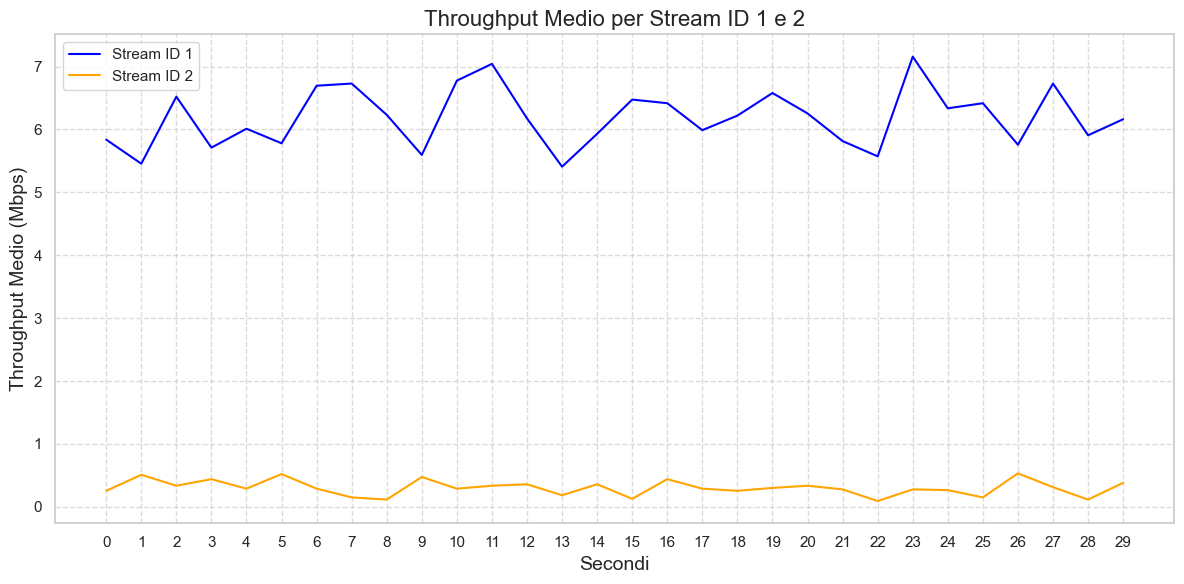
\includegraphics[width=\textwidth]{t2_c2_main.png} % Sostituisci con il path del grafico
        \end{minipage}
    \end{minipage}

\end{frame}


\begin{frame}
    \frametitle{COnclusioni test}
\end{frame}

\begin{frame}
    \frametitle{COnclusioni finali}
\end{frame}

\begin{frame}
    \frametitle{The end}
\end{frame}

\end{document}
